\subsection{Исходное изображение}

Обратимся к кругам и их производным. Исходное изображение:

\begin{figure}[ht!]
    \centering
    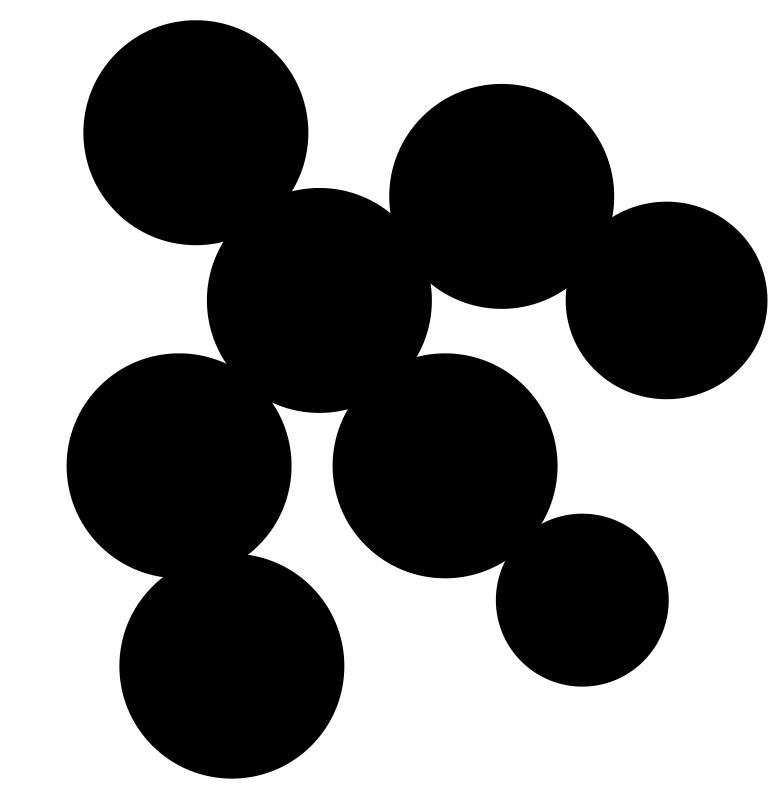
\includegraphics[width=0.5\textwidth]{images/source_images/circles.jpg}
    \caption{Круги}
    \label{img:circles_orig}
\end{figure} 

Для выполнения этого задания воспользуемся \textit{MATLAB}.

\subsection{Программа на языке MATLAB}

\begin{lstlisting}[caption={Исходный код программы для разделения объектов}, label={lst:separation}]
    src_img = imread("circles.jpg");
    gray_img = im2gray(src_img);
    BW = imbinarize(gray_img);
    BW = ~BW;
    imwrite(BW,"binary_inv.jpg");
    BW2 = bwmorph(BW,'erode',45);
    imwrite(BW2,"erosed.jpg");
    BW2 = bwmorph(BW2,'thicken',Inf);
    imwrite(BW2,"boundaries.jpg");
    BW = ~(BW & BW2);
    imwrite(BW,"result.jpg");
\end{lstlisting}

\subsection{Результаты}
\vspace{3cm}
\begin{figure}[ht!]
    \centering
    \begin{subfigure}{0.4\textwidth}
        \centering
        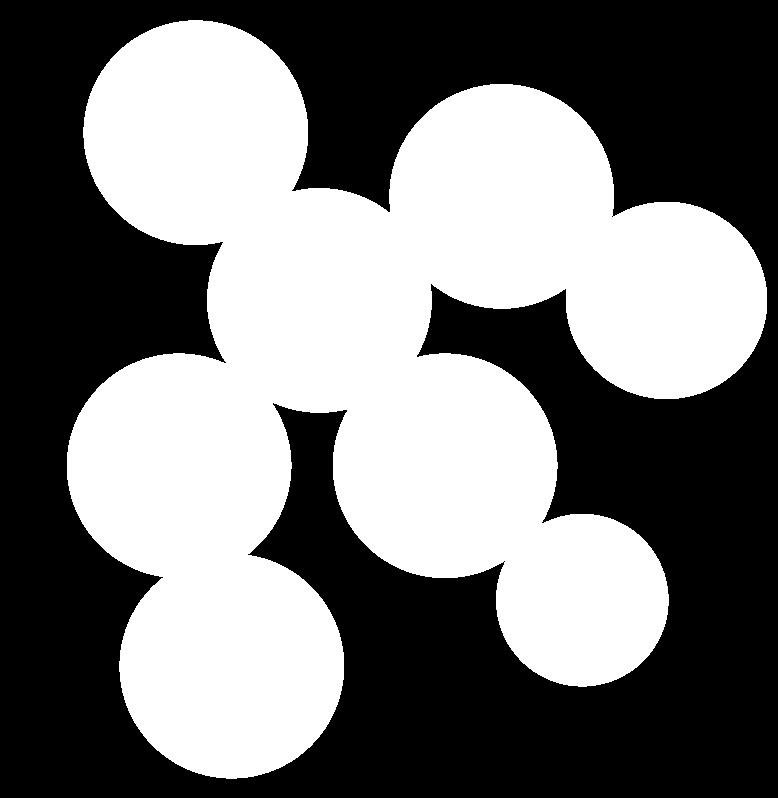
\includegraphics[width=\textwidth]{images/transformed_images/2/binary_inv.jpg}
        \caption{}
        \label{img:bin_inv}
    \end{subfigure}
    \begin{subfigure}{0.4\textwidth}
        \centering
        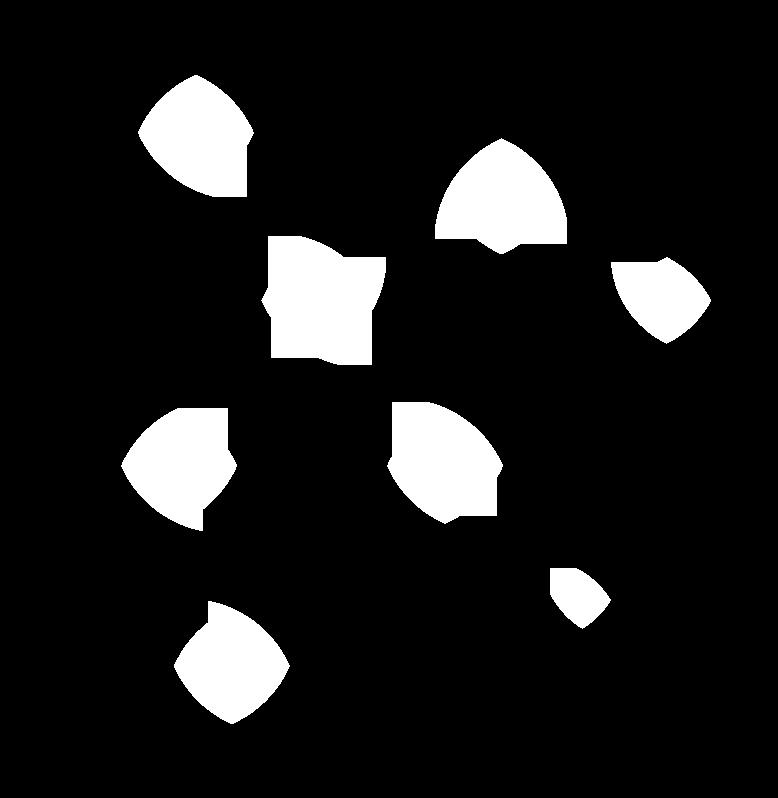
\includegraphics[width=\textwidth]{images/transformed_images/2/erosed.jpg}
        \caption{}
        \label{img:erosed_circles}
    \end{subfigure}
    \begin{subfigure}{0.4\textwidth}
        \centering
        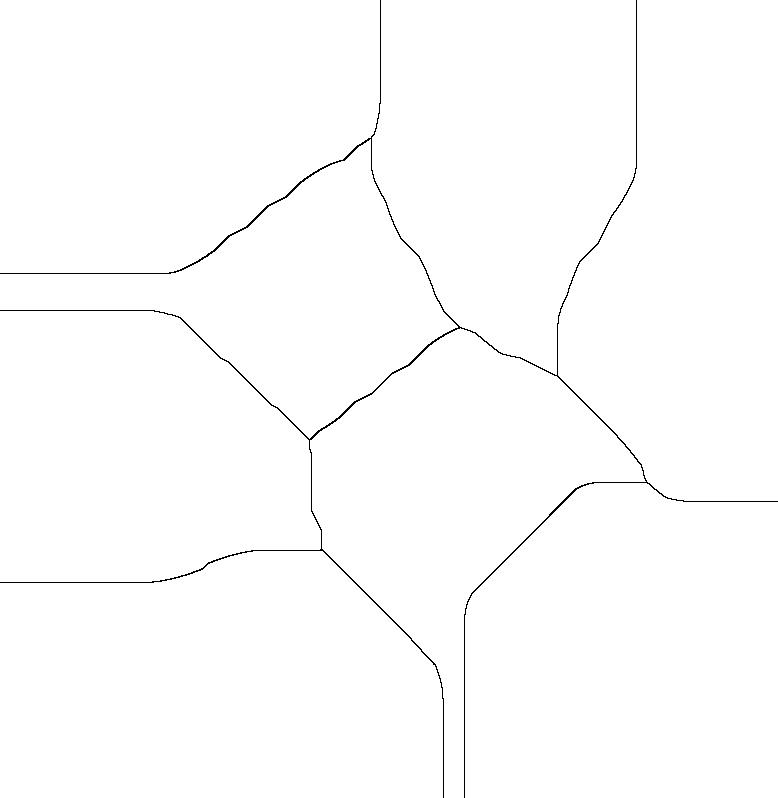
\includegraphics[width=\textwidth]{images/transformed_images/2/boundaries.jpg}
        \caption{}
        \label{img:boudaries}
    \end{subfigure}
    \begin{subfigure}{0.4\textwidth}
        \centering
        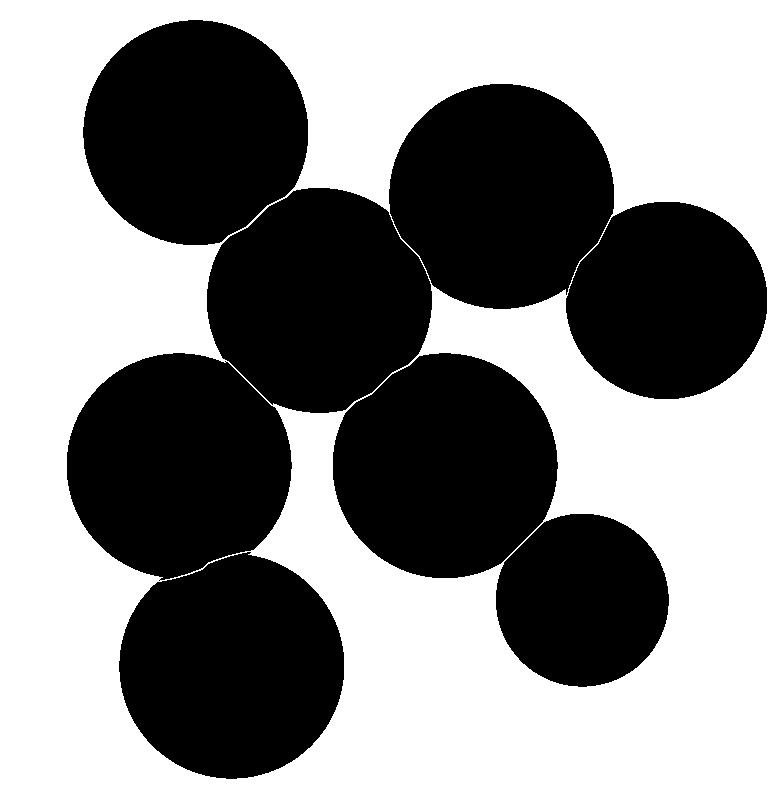
\includegraphics[width=\textwidth]{images/transformed_images/2/result.jpg}
        \caption{}
        \label{img:result_circles}
    \end{subfigure}
    \caption{Разделение <<склееных объектов>>: (а) инвертированное бинарное изображение, (b) эрозия бинарного изображения, (c) расширение объектов, (d) результат разделения}
    \label{img:Cirlces}
\end{figure}